\section{Q1: Why does an MLP do badly on CIFAR-10?}
\label{sec:q1}

\subsection{(a) Missing spatial prior or missing capacity?}
\textbf{Hypothesis.} An MLP treats the $3\times32\times32$ input as an unordered vector of 3072 numbers. It has
no notion that neighbouring pixels belong together or that a pattern means the same thing wherever it appears,
so it must learn locality and shift invariance from 45k images. Our claim is that it cannot, and that it ends
up \emph{fitting} the training set without generalising. The competing explanation is that the MLP is simply
too small or too hard to optimise, i.e.\ it \emph{underfits}.

\textbf{Design.} The two explanations make different predictions. Under the capacity explanation the MLP has low
training accuracy and more parameters raise validation accuracy clearly. Under the spatial-prior explanation the
MLP reaches high training accuracy, extra width barely helps, and a network with the prior built in does much
better at the \emph{same} parameter count and training budget. Four models were trained
(Tab.~\ref{tab:q1a}): a base MLP, a CNN with the same number of parameters, an MLP with 4.25$\times$ the
parameters (capacity test), and the base MLP with random flips and 4-pixel crops, which gives some shift
invariance through the data instead of the architecture. Both networks use BatchNorm and ReLU so neither gets a
normalisation advantage. The CNN is six $3\times3$ convolutions (64, 64, 128, 128, 256, 256 channels; max
pooling after the second and fourth), global average pooling and one linear layer.

\textbf{Fairness.} Parameters are matched to 0.14\%, epochs, optimiser, schedule, batch size, seed and
learning-rate grid are identical, and the learning rate is chosen on validation for each model. What is not
matched is computation per step: the CNN reuses each filter at every position and therefore performs many
more multiply-adds per parameter. We regard this as part of what the spatial prior is, not as an extra
advantage, but note it.

\begin{table}[t]
\centering
\small
\begin{tabular}{@{}lrcccc@{}}
\toprule
Model & Params & lr & Train & Val & Test \\
\midrule
MLP 3072-336-336-10 & 1{,}150{,}474 & 0.3 & 0.971 & 0.578 & 0.573 \\
Wide MLP 3072-1152-1152-10 & 4{,}884{,}490 & 0.1 & 1.000 & 0.600 & 0.587 \\
MLP + flip/crop & 1{,}150{,}474 & 0.1 & 0.664 & 0.615 & 0.621 \\
CNN (6 conv + GAP + FC) & 1{,}148{,}874 & 0.3 & 1.000 & 0.900 & \textbf{0.897} \\
\bottomrule
\end{tabular}
\caption{Q1(a). Selected learning rate, final-epoch train/val accuracy and the single test evaluation.}
\label{tab:q1a}
\end{table}

\begin{figure*}[t]
\centering
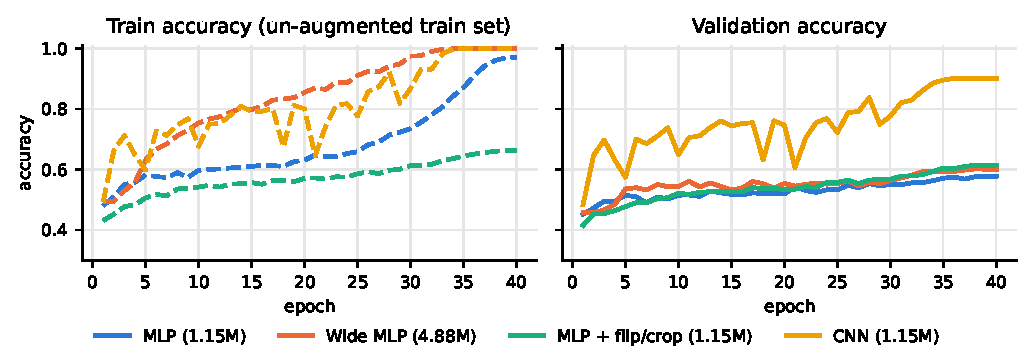
\includegraphics[width=\textwidth]{q1a_curves}
\caption{Q1(a) training curves of the selected runs. Train accuracy (left, dashed) and validation accuracy
(right). The MLPs reach (near) 100\% train accuracy while validation stays at 0.58--0.62.}
\label{fig:q1a}
\end{figure*}

\textbf{Result.} Capacity is not the bottleneck: the base MLP fits 97\% of the training set and the wide one
100\% (Fig.~\ref{fig:q1a}), yet 4.25$\times$ more parameters add only 1.4 test points. The train--val gap (0.39)
is the problem, not the training error. With the same parameter budget the CNN reaches 0.897 on test,
+32 points. Augmentation narrows the MLP's gap a lot (train 0.66 vs val 0.61) and adds 4.9 test points, so
small-shift invariance is part of the story, but the MLP stays 28 points behind. The evidence points to the
missing locality and weight sharing, which the MLP cannot learn from 45k images, rather than to underfitting.

\subsection{(b) Structure before memorisation}
\textbf{Setting.} 20\% of the 45k training labels were replaced by a different class chosen uniformly from the
other nine (seed 242003). Nothing in an image predicts its new label, so these examples cannot generalise and
can only be fitted by memorising them. The MLP was made large (3072-2048-2048-10, 10.5M parameters, about 230
per training image) and nothing discourages memorisation: no weight decay, no augmentation, constant learning
rate 0.002 (so changes in the curves are not caused by a schedule), 60 epochs. Two pilots (learning rate 0.01
and 0.002, one measurement per epoch) showed that everything happens in the first ~20 epochs, so the final runs
measure eight times per epoch. Runs with 0\% and 40\% relabelled examples serve as controls.

\textbf{Measurements across training.} At every measurement we record (i) accuracy on correctly labelled
training images, (ii) the fraction of relabelled images predicted as their \emph{wrong} training label
(memorisation), (iii) the fraction of relabelled images predicted as their \emph{true} class, and (iv) validation
accuracy (Fig.~\ref{fig:q1b}, Tab.~\ref{tab:q1b}).

\begin{figure*}[t]
\centering
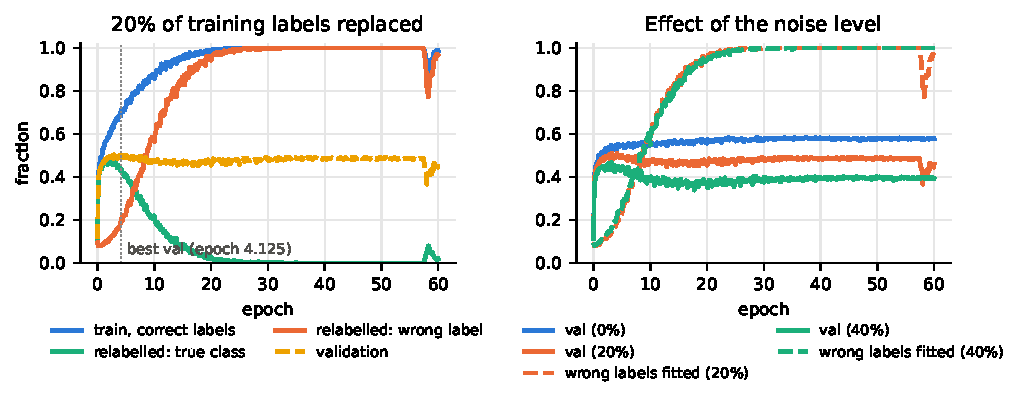
\includegraphics[width=\textwidth]{q1b_memorisation}
\caption{Q1(b). Left: 20\% relabelled. In the first epochs about 47\% of the relabelled training images are
predicted as their true class although the network is trained towards another label; validation peaks at
epoch 4.1, before the wrong labels overtake the true ones (epoch 6.5). Right: the same for 0/20/40\%. The dip
near epoch 58 is a single loss spike of the constant-lr run and is recovered within an epoch.}
\label{fig:q1b}
\end{figure*}

\begin{table}[t]
\centering
\small
\begin{tabular}{@{}rcccc@{}}
\toprule
Epoch & Train (correct) & Relab.$\to$true & Relab.$\to$wrong & Val \\
\midrule
1 & 0.534 & 0.461 & 0.086 & 0.471 \\
3 & 0.652 & 0.471 & 0.132 & 0.497 \\
4.1 & 0.710 & 0.439 & 0.190 & \textbf{0.512} \\
8 & 0.818 & 0.284 & 0.431 & 0.479 \\
15 & 0.952 & 0.088 & 0.837 & 0.459 \\
30 & 1.000 & 0.000 & 1.000 & 0.478 \\
\midrule
\multicolumn{5}{@{}l}{Test acc.\ (best-val checkpoint / final): 0\%: 0.565 / 0.564;} \\
\multicolumn{5}{@{}l}{20\%: 0.503 / 0.457;\quad 40\%: 0.459 / 0.395} \\
\bottomrule
\end{tabular}
\caption{Q1(b), 20\% relabelled. Bottom: test accuracy of the checkpoint with the best validation accuracy
(selected on validation) and of the final, memorising model.}
\label{tab:q1b}
\end{table}

\textbf{Interpretation.} Useful structure is learned first. In the first three epochs the network predicts the
\emph{true} class for 47\% of the relabelled images while being pushed towards a different label; it can only do
this with features that transfer across images, and validation accuracy rises at the same time. Memorisation
starts afterwards: the wrong-label fit grows from 0.13 (epoch 3) to 0.43 (epoch 8) and 1.00 (epoch 30), the
true-class fraction collapses, and validation drops from its peak of 0.512 at epoch 4.1. The peak comes before
the crossover at epoch 6.5. With clean labels, validation keeps improving until epoch 29 and does not fall, so
the drop in the noisy runs comes from fitting the wrong labels, not from long training as such; at 40\% noise the
peak and the crossover come earlier and the drop is larger. On test, early stopping on validation keeps 4.6
(20\%) and 6.3 (40\%) points that the memorising model loses, while with clean labels the two coincide. This
agrees with the ordering reported by Arpit~\etal~\cite{arpit2017closer} and with the observation that such
networks can fit random labels~\cite{zhang2017rethinking}.
